\chapter{Methodology}

    % \fei{You cannot use his work, but have to write in your own words.  If you are going to talk about AnDri which is not your work, then describe this in Background chapter.  Move 3.2 to Background. }
    % \fei{Describe your methodology using a picture to show what is the problem, and then a picture showing your solution (framework).  This chapter is all about the algorithm details so show using a picture and explain how your algorithm works.  I don't  understand how 3.5 is an algorithm method.}
    % \fei{Why is this interesting as an algorithm?  }

This chapter describes the methodological workflow used in this project. The focus here is the end-to-end detection methodology implemented in the demo system: score generation, normal-pattern-aware thresholding, active-learning-based label refinement, and final anomaly decision making. While anomaly scores and normal-pattern assignments are obtained from existing detectors such as AnDri, the adaptive threshold refinement framework, Bayesian mixture-based threshold estimation, active-learning candidate selection strategy, and pattern-specific threshold assignment were designed and implemented in this project.


\section{Problem Definition}

Let \(T=[x_1,x_2,\ldots,x_n]\) be a uni-variate time series, where \(x_i\) is the observed value at time index \(i\). The goal of anomaly detection is to decide whether each time point is normal or anomaly. Anomaly detection method first assigns each time point an anomaly score \(s_i\), and a larger score means that the point is more suspicious.

The detector therefore transforms the original time series into a point-level anomaly-score sequence:
\[S=[s_1,s_2,\ldots,s_n].\]
Here, each point \(i\) has an anomaly score \(s_i\).

After the anomaly scores are generated, a threshold is applied to decide the final anomaly label (anomaly or normal points)
\[
\hat{y}_i =
\begin{cases}
1, & \text{if } s_i > \theta,\\
0, & \text{otherwise,}
\end{cases}
\]
where \(\hat{y}_i=1\) means that point \(i\) is predicted as anomaly, and \(\hat{y}_i=0\) means that it is predicted as normal point. This workflow is common in time-series anomaly detection. Time series anomaly detect methods produce anomaly scores. Final anomaly labels will depend on how the threshold is selected.

Concept drift complicates threshold selection because normal behavior changes over time. A fixed threshold may therefore produce false positives or miss true anomalies. AnDri system addresses this problem by supporting interactive threshold adjustment. The user can review candidate anomalous points, provide feedback. So that the system can refine the threshold according to the user feedback to convert anomaly scores into final labels. This feedback process is important in the system because both AnDri and the baseline methods generate point anomaly scores, and a threshold must be proposed and refined to predict the final decision.

Figure~\ref{fig41} illustrates this problem formulation. The upper plot shows the original time series. The lower plot shows the anomaly score of each time point. The threshold is applied to the anomaly-score curve.

\begin{figure}[H]
\centering
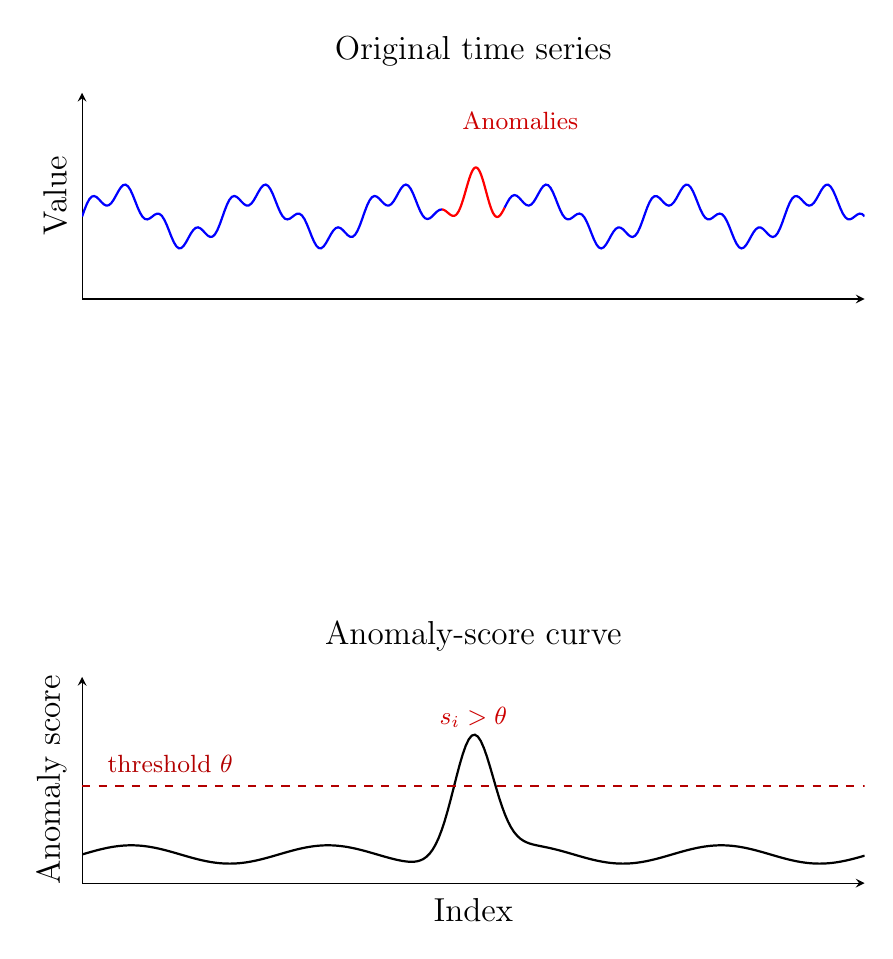
\begin{tikzpicture}
\begin{axis}[
    name=rawseries,
    width=0.95\textwidth,
    height=4.2cm,
    xmin=0, xmax=100,
    ymin=-1.6, ymax=2.4,
    axis lines=left,
    xtick=\empty,
    ytick=\empty,
    ylabel={Value},
    title={Original time series},
    label style={font=\large},
    title style={font=\large}
]


\def\series{0.45*sin(deg(0.35*x))+ 0.20*sin(deg(1.4*x))+ 1.2*exp(-0.15*(x-50)^2)}

\addplot[
    blue,
    thick,
    domain=0:46,
    samples=150
]
{\series};


\addplot[
    red,
    thick,
    domain=46:54,
    samples=120
]
{\series};

\addplot[
    blue,
    thick,
    domain=54:100,
    samples=150
]
{\series};

\node[
    red!80!black,
    font=\small
] at (axis cs:56,1.85)
{Anomalies};

\end{axis}

\begin{axis}[
    name=scoreseries,
    at={(rawseries.south west)},
    yshift=-4.8cm,
    anchor=north west,
    width=0.95\textwidth,
    height=4.2cm,
    xmin=0, xmax=100,
    ymin=0, ymax=1.8,
    axis lines=left,
    xlabel={Index},
    ylabel={Anomaly score},
    xtick=\empty,
    ytick=\empty,
    title={Anomaly-score curve},
    label style={font=\large},
    title style={font=\large}
]
\addplot[black, thick, domain=0:100, samples=260]
{0.25 + 0.08*sin(deg(0.25*x)) + 1.05*exp(-0.08*(x-50)^2)};

\addplot[dashed, red!70!black, thick] coordinates {(0,0.85) (100,0.85)};

\node[red!70!black, font=\small, anchor=south west] at (axis cs:2,0.88) {threshold \(\theta\)};
\node[red!80!black, font=\small] at (axis cs:50,1.45) {\(s_i > \theta\)};
\end{axis}

\end{tikzpicture}
\caption{ Each point in the original time series is assigned an anomaly score, and the threshold is applied to the anomaly-score curve to obtain final anomaly labels.}
\label{fig41}
\end{figure}




\section{Method Overview}

The implemented workflow has four main stages. First, the system converts the input time series into anomaly scores. For AnDri, this stage also returns the normal pattern associated with each point. Second, the user selects one or more training regions and marks a small number of anomalies. Third, the system estimates anomaly thresholds from the score distribution of the user-labeled points. Fourth, when the score distribution is ambiguous, the system requests additional user feedback for candidate points and updates the threshold iteratively.


\section{Anomaly Score Generation}

Anomaly detect algorithms mentioned in this report generate anomaly scores for each data point
\[S=[s_1,s_2,\ldots,s_n],\]
where a larger score indicates stronger evidence of abnormality. In the implementation, scores are normalized to the interval \([0,1]\).

AnDri algorithm also assigns each point to a normal pattern index:
\[g(i) \in \{1,2,\ldots,m\},\]
where \(g(i)\) indicates the normal pattern that best matches point \(i\). 


\section{Overall Workflow}

The overall methodology can be summarized as follows.

\begin{figure}[H]
\centering
\begin{tikzpicture}[
    font=\scriptsize,
    node distance=0.6cm and 1.15cm,
    process/.style={
        rectangle,
        rounded corners,
        draw,
        align=center,
        text width=4.1cm,
        minimum height=0.85cm
    },
    smallprocess/.style={
        rectangle,
        rounded corners,
        draw,
        align=center,
        text width=2.65cm,
        minimum height=0.85cm
    },
    decision/.style={
        diamond,
        draw,
        aspect=2.1,
        align=center,
        inner sep=1pt,
        text width=2.55cm
    },
    arrow/.style={-{Latex}, thick }
]

\node[process] (input)
{Input time series \(T\), training regions, partial user labels, and anomaly proportion \(\rho\)};

\node[process, below=of input] (score)
{Compute normalized anomaly scores \(S=[s_1,\ldots,s_n]\)};

\node[decision, below=of score] (method)
{Using AnDri?};

\node[smallprocess, right=of method] (andri)
{Use normal-pattern assignment\\
\(g(i)\) for each point};

\node[smallprocess, below=of andri] (andrigroup)
{Form pattern-specific groups 
\(A_k=\{i\in A \mid g(i)=k\}\)};

\node[process, below=of method] (baselinegroup)
{Form one global threshold group};

\node[process, below=1.0cm of baselinegroup] (fit)
{Fit or refit Bayesian Gaussian mixture to current user-marked anomaly scores};

\node[decision, below=of fit] (stable)
{Stable score distribution?};

\node[smallprocess, right=of stable] (query)
{Select review candidates:\\
low-score marked anomalies or\\
points near Gaussian intersection};

\node[smallprocess, below=of query] (feedback)
{User confirms candidates as anomaly or normal};

\node[smallprocess, below=of feedback] (update)
{Update labels};

\node[process, below=of stable] (threshold)
{Set threshold for this group\\
\(\theta=\max(q_{\rho},\mu-\sigma)\)};

\node[decision, below=of threshold] (more)
{More groups\\to process?};

\node[process, below=of more] (label)
{Assign final labels using each point's group threshold\\
\(\hat{y}_i=1\) if \(s_i>\theta_{c(i)}\)};

\draw[arrow] (input) -- (score);

\draw[arrow] (score) -- (method);

\draw[arrow] (method) -- node[above] {yes} (andri);

\draw[arrow] (andri) -- (andrigroup);

\draw[arrow] (andrigroup.south) |- ([yshift=10pt]fit.east);

\draw[arrow] (method) -- node[left] {no} (baselinegroup);

\draw[arrow] (baselinegroup) -- (fit);

\draw[arrow] (fit) -- (stable);

\draw[arrow] (stable) -- node[left] {yes} (threshold);
\draw[arrow] (stable) -- node[above] {no} (query);

\draw[arrow] (query) -- (feedback);

\draw[arrow] (feedback) -- (update);
\draw[arrow] (update.east) -- ++(1.2,0) |- ([yshift=-8pt]fit.east);
\draw[arrow] (threshold) -- (more);
\draw[arrow] (more) -- node[left] {no} (label);

\draw[arrow] (more.west) -- ++(-1.15,0) node[left] {yes} |- (fit.west);

\end{tikzpicture}
\caption{Workflow Overview.}
\label{fig42}

\end{figure}


This methodology connects the algorithmic score output with the interactive system workflow. The backend produces normalized scores and, for AnDri, normal-pattern assignments. The frontend uses those values to guide user to review and then present final decisions. In this way, the system does not rely only on a static cutoff. Instead, it uses partial human feedback to adapt the decision boundary and uses AnDri's normal-pattern structure to make the threshold sensitive to concept drift.



\section{Dynamic Threshold Setting with User Feedback}

After anomaly scores are generated, the key methodological step is to convert the continuous score sequence into binary anomaly labels. The system combines an initial anomaly-proportion estimation, user-marked anomaly points, Bayesian mixture fitting, and candidate review to dynamically refine the final decision threshold.

Let \(\rho \in [0,1]\) be the maximum allowable anomaly proportion specified by the user. This parameter provides a proportion-based constraint during threshold estimation. For example, when \(\rho=0.05\), it means that at most \(5\%\) of points with the highest anomaly scores would be classified as anomalies in the final stage.

At the beginning of the interaction, the user marks anomaly points. The system maintains a label state
\[
f_i =
\begin{cases}
0, & \text{unlabeled},\\
1, & \text{user-confirmed anomaly},\\
2, & \text{user-confirmed normal}.
\end{cases}
\]
Only the scores of user-confirmed anomalies are used to estimate the anomaly-score distribution. Points with \(f_i=2\) are not used as normal training examples for fitting the Bayesian model; they are removed from the candidate anomaly set and excluded from future uncertain-candidate queries. They are regarded as erroneous labels made by the users.

Given the current confirmed anomaly set \(L=\{i\in A\mid f_i=1\}\), the backend fits a two-component Bayesian Gaussian mixture model to the marked anomalies' scores:
\[
p(s)=\sum_{k=1}^{2}\pi_k\mathcal{N}(s;\mu_k,\sigma_k^2).
\]

It is worth noting here that the Bayesian Gaussian mixture model is not used to separate normal and anomalous points. It is applied to the scores of user-confirmed anomalies to assess whether the labeled anomalies form a stable single distribution or multiple competing score groups.

A component is treated as active only when its mixture weight is larger than a small weight threshold. If the Bayesian mixture has only one active components, the marked anomaly scores are considered stable. The threshold is then set as
\[
\theta=\max(\theta_{\rho},\mu_a-\sigma_a),
\]
where \(\mu_a\) and \(\sigma_a\) are the mean and standard deviation of the stable active anomaly-score component.

If two active components remain, the system regards the current threshold as uncertain. It then selects candidate points for user review in two ways. First, if a user-marked anomaly has a score below \(\theta_{\rho}\), the system asks the user whether this point should remain an anomaly. This step removes possible low-score mislabels. Second, the system finds the intersection region between the two active Gaussian components and asks the user to confirm unlabeled points near this uncertain boundary. If the user confirms a candidate, its flag becomes \(f_i=1\); if the user rejects it, its flag becomes \(f_i=2\). After each review round, the Bayesian mixture is refitted and the threshold is updated.

For the baseline detectors, including NormA, SAND, and DAMP, this process produces one global threshold. For AnDri, the same threshold-setting procedure is applied separately to each normal-pattern group in the selected training region. Let \(g(i)\) be the normal-pattern index assigned to point \(i\). For pattern \(k\), the training subset is
\[
A_k=\{i\in A\mid g(i)=k\}.
\]
The system estimates a pattern-specific threshold \(\theta_k\) using only the scores and user feedback associated with \(A_k\). The final AnDri prediction is
\[
\hat{y}_i =
\begin{cases}
1, & s_i>\theta_{g(i)},\\
0, & s_i\leq \theta_{g(i)}.
\end{cases}
\]
If a test point belongs to a normal pattern that was not present in the selected training region, the system assigns the threshold of the most similar trained normal pattern, measured by Euclidean distance between normal-pattern subsequences.



\begin{figure}[H]
\centering
\begin{tikzpicture}[
    flowbox/.style={
        rectangle,
        draw,
        thick,
        rounded corners=1pt,
        fill=blue!25,
        minimum width=6.4cm,
        minimum height=0.75cm,
        align=center,
        font=\small
    },
    note/.style={font=\small, align=left},
    arrow/.style={-{Latex}, thick},
    callout/.style={densely dashed, blue!70!black, thick}
]

\node[flowbox] (p1) {1. Set anomaly proportion \(\rho\)};
\node[flowbox, below=0.85cm of p1] (p2) {2. Mark initial anomaly points};
\node[flowbox, below=0.85cm of p2] (p3) {3. Fit Bayesian mixture to marked anomaly scores};
\node[flowbox, below=0.85cm of p3] (p4) {4. Review uncertain candidate points};
\node[flowbox, below=0.85cm of p4] (p5) {5. Finalize threshold and anomaly labels};

\draw[arrow] (p1) -- (p2);
\draw[arrow] (p2) -- (p3);
\draw[arrow] (p3) -- (p4);
\draw[arrow] (p4) -- (p5);

\draw[callout] (p1.east) -- ++(1.0,0)
node[note, right, black] {Top \(\rho\) score cutoff};
\draw[callout] (p3.east) -- ++(1.0,0)
node[note, right, black] {Bayesian Gaussian mixture};
\draw[callout] (p4.east) -- ++(0.8,0) |- ++(0.35,0.35)
node[note, right, black] {Low-score marked anomalies};
\draw[callout] (p4.east) -- ++(0.8,0) |- ++(0.35,-0.35)
node[note, right, black] {Scores near mixture intersection};

\end{tikzpicture}
\caption{Overview of dynamic threshold setting with user feedback.}
\label{fig:dynamic_threshold_overview}
\end{figure}